% Generated by thesis/ch7/exp1/churn_case_figures.py -- do not edit by hand.
\begin{figure}[tbp]
  \centering
  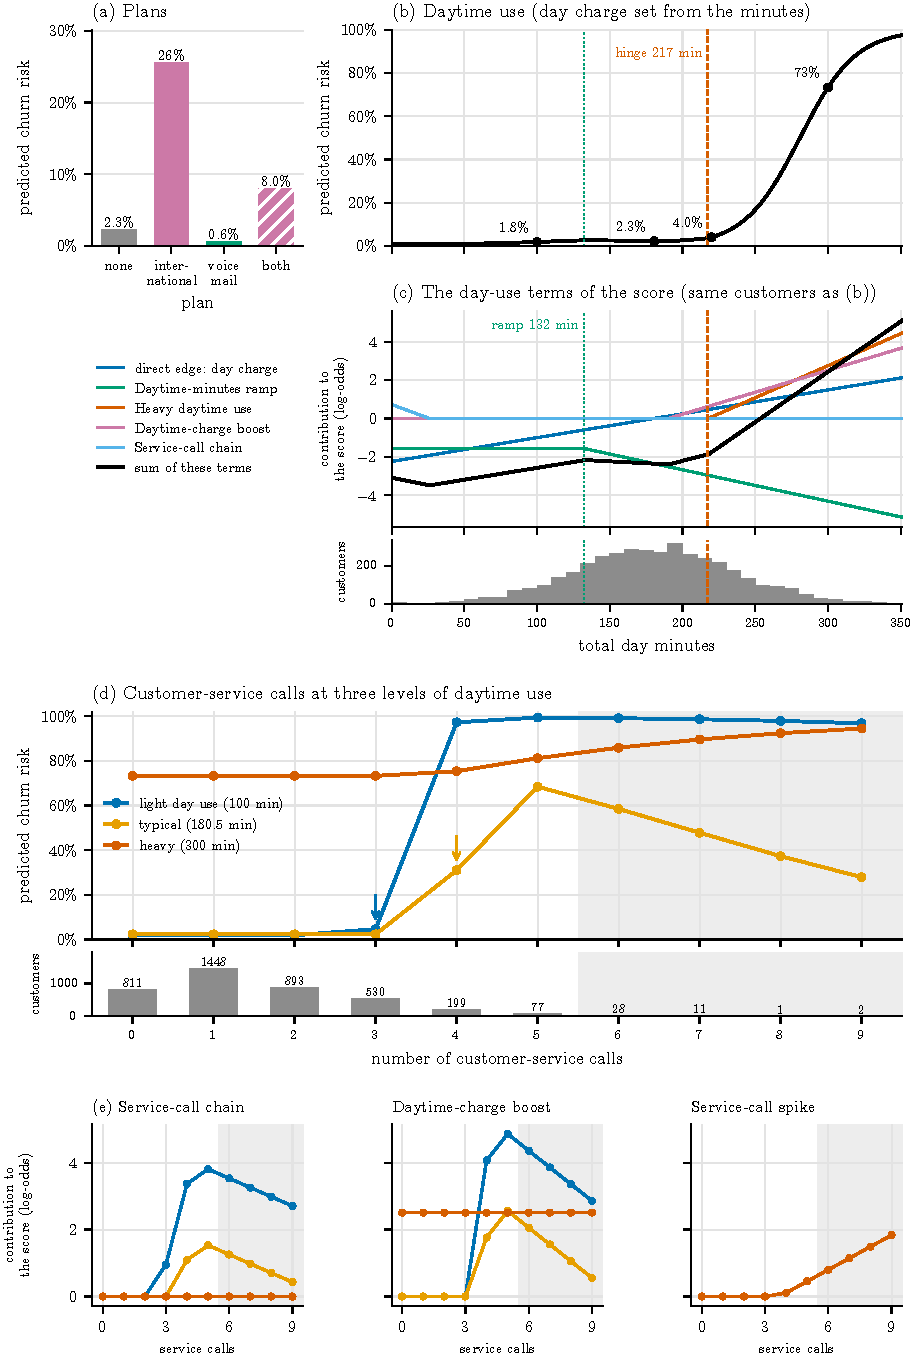
\includegraphics[width=\textwidth,height=0.85\textheight,keepaspectratio]{figures/ch7/churn-case-probes.pdf}
  \caption{Churn case network (seed 10): predicted churn risk of the typical customer as inputs change. (a) The plans (hatched: both). (b) Black: risk against daytime use, the day charge set from the minutes; dots: 100, 180.5, 220, 300 minutes; dashed red: where the part \emph{Heavy daytime use} switches on; grey bars: training customers per 10 minutes. (c) Risk against customer-service calls at three levels of daytime use (colours); arrow: the call count at which the part \emph{Service-call chain} switches on; grey bars: training customers per call count; shaded: fewer than 50 training customers. (d) The three service-call parts' contributions to the score (log-odds) over the same calls, colours as in (c); a line not visible lies under another.}
  \label{fig:ch7-churn-case-probes}
\end{figure}
